This section reviews some programming languages and how they provide ``freedom from choice'', in the sense of A. Sangiovani-Vincentelli~\cite{lee2019freedom}.
There is a distinct sense in this is the central question of programming languages in general.
By removing memory managment through having no pointer arithmetic and gargabe collection, Java frees its users from multiple families of errors that are possible in C.
Rust's ownership types take a different approach, also removing complete families of memory-management based errors, without introducing large performance overheads or unpredicatble behavior from the gargabe collector.
These kinds of ``freedom from choice'' in general-purpose languages are beyond the scope of this thesis, which focuses on \acp{MoC} like those described in Chapter~\ref{chap:mocs}.
As such, we will survey languages focused on these paradigms.

\subsection{Dataflow and Actors}

Discuss commercial ones.

Most well-known languages that follow \acp{MoC} like the ones described here are based on the actor model.
Compared to more sophisticated

CPN

CAL

Ptolemy
\begin{figure}[t]
	\centering
	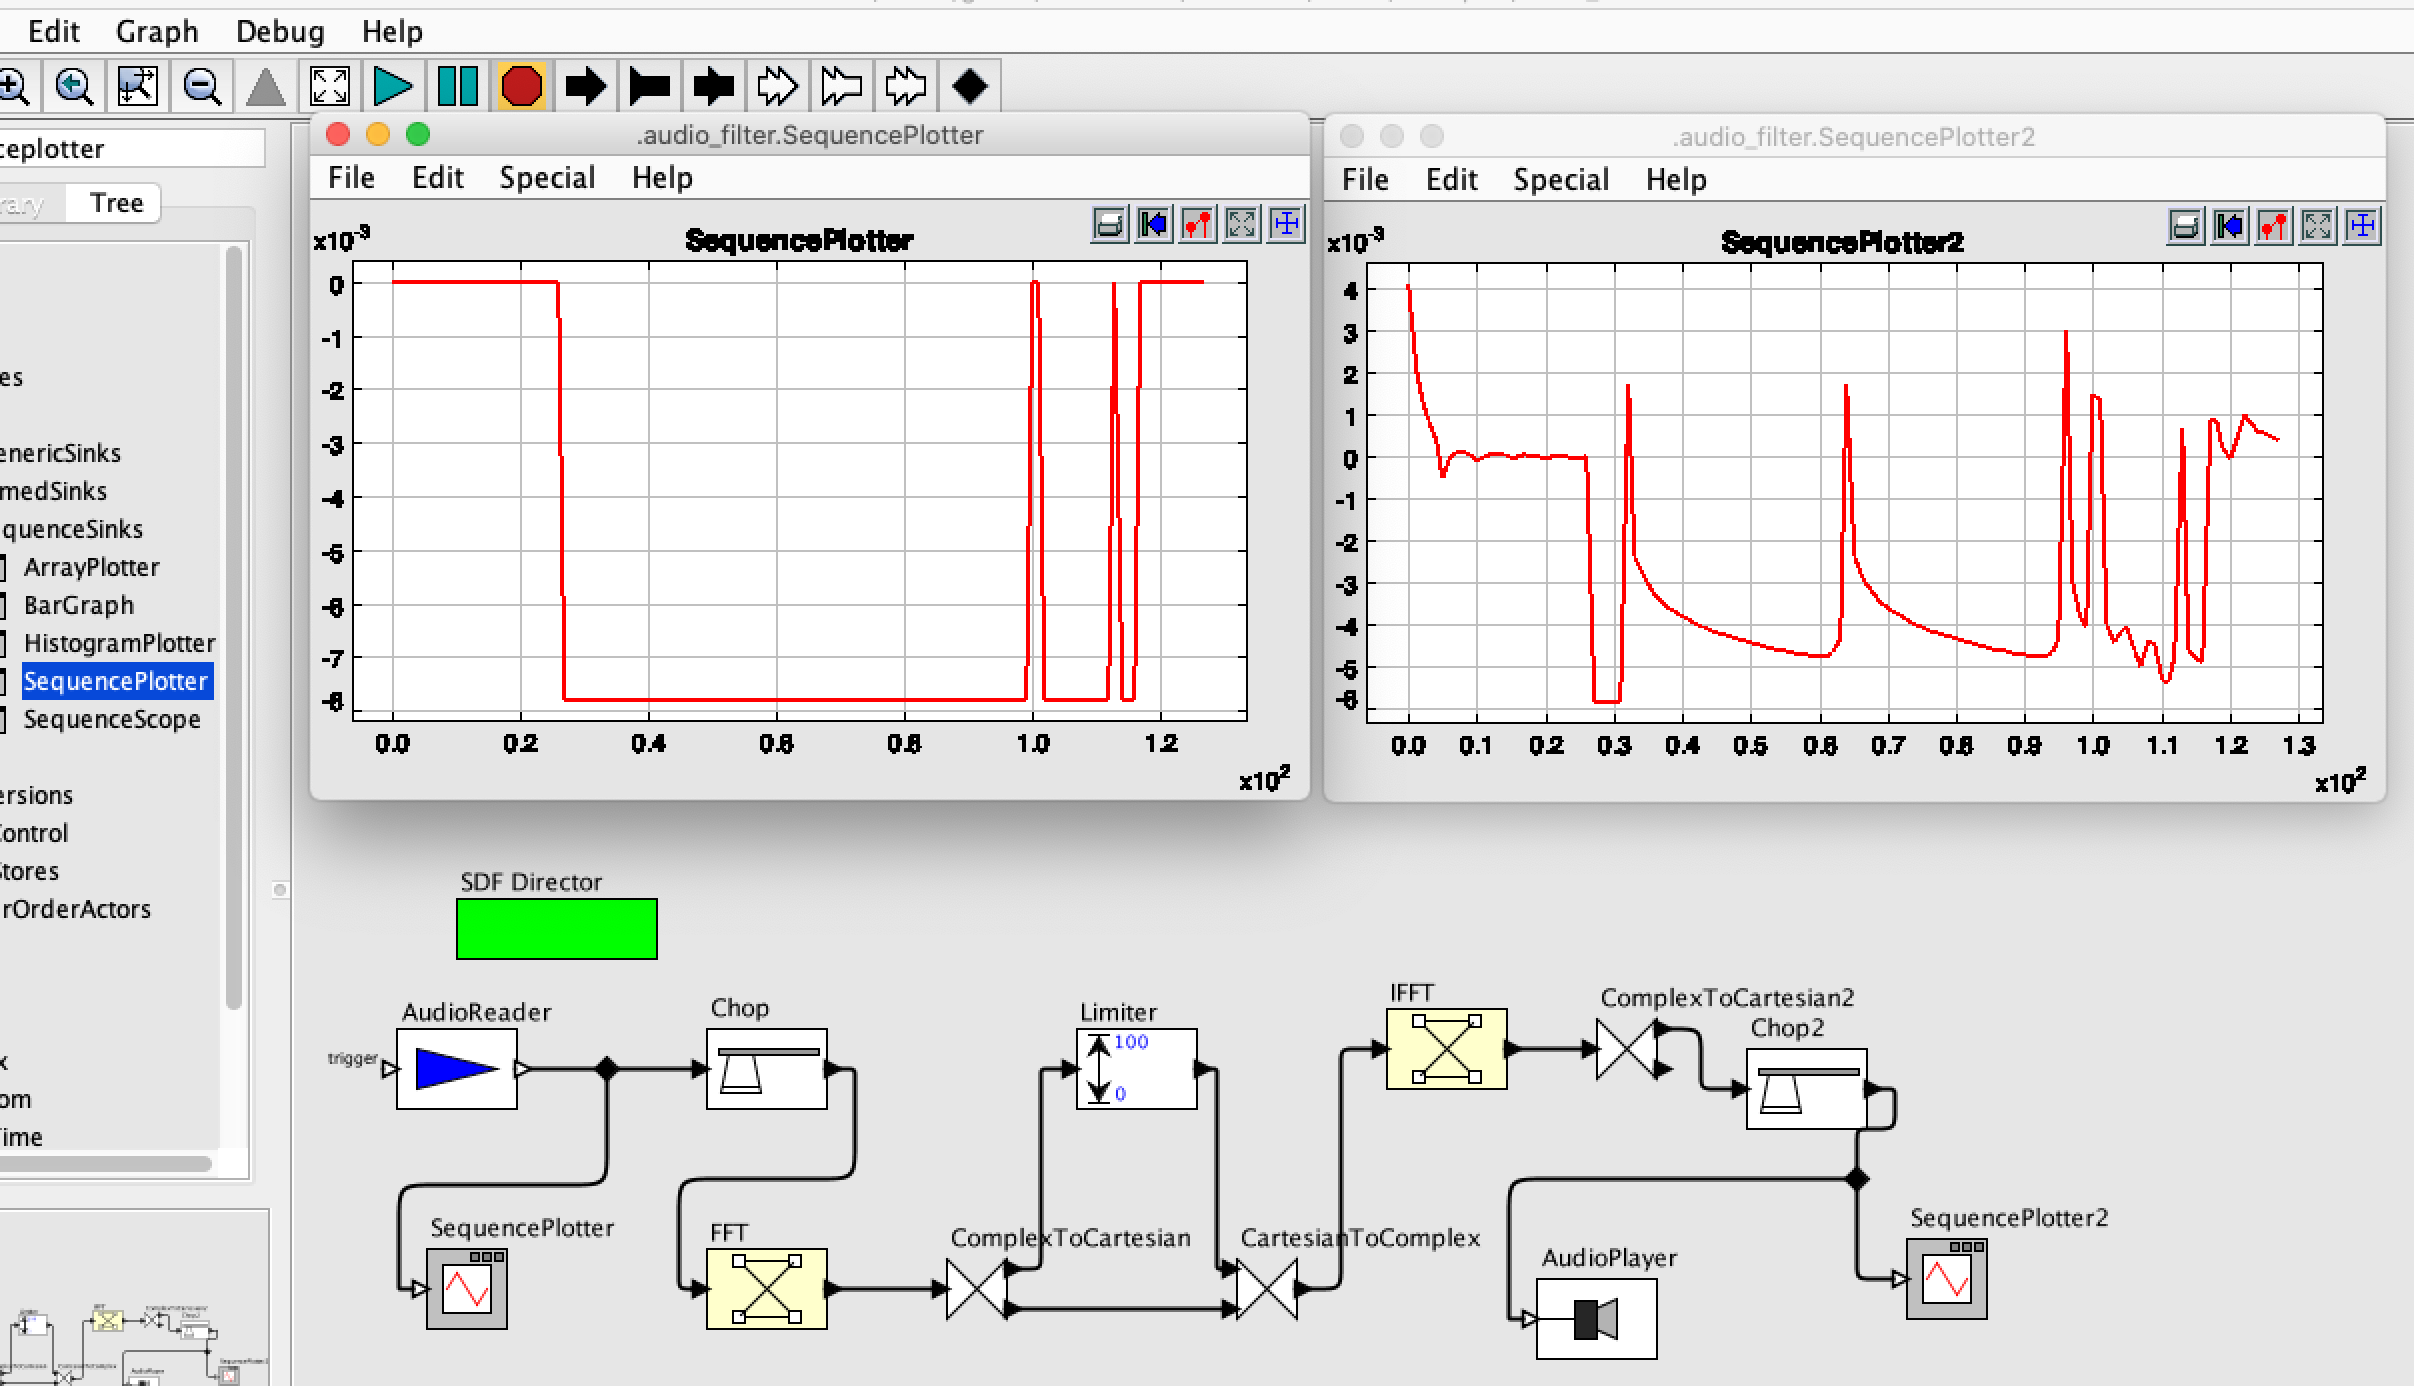
\includegraphics[width=0.9\textwidth]{figures/audio_filter_ptolemy_screenshot.png}
	\caption{An audio filter in \ac{SDF} semantics in Ptolemy II}
	\label{fig:audio_filter_ptolemy}
	%	\vspace{-1mm}
\end{figure}

The one from Pimientel

\subsection{Discrete-Events Languages}

Synchronous languages

SystemC

Lingua Franca
\begin{figure}[t]
	\centering
	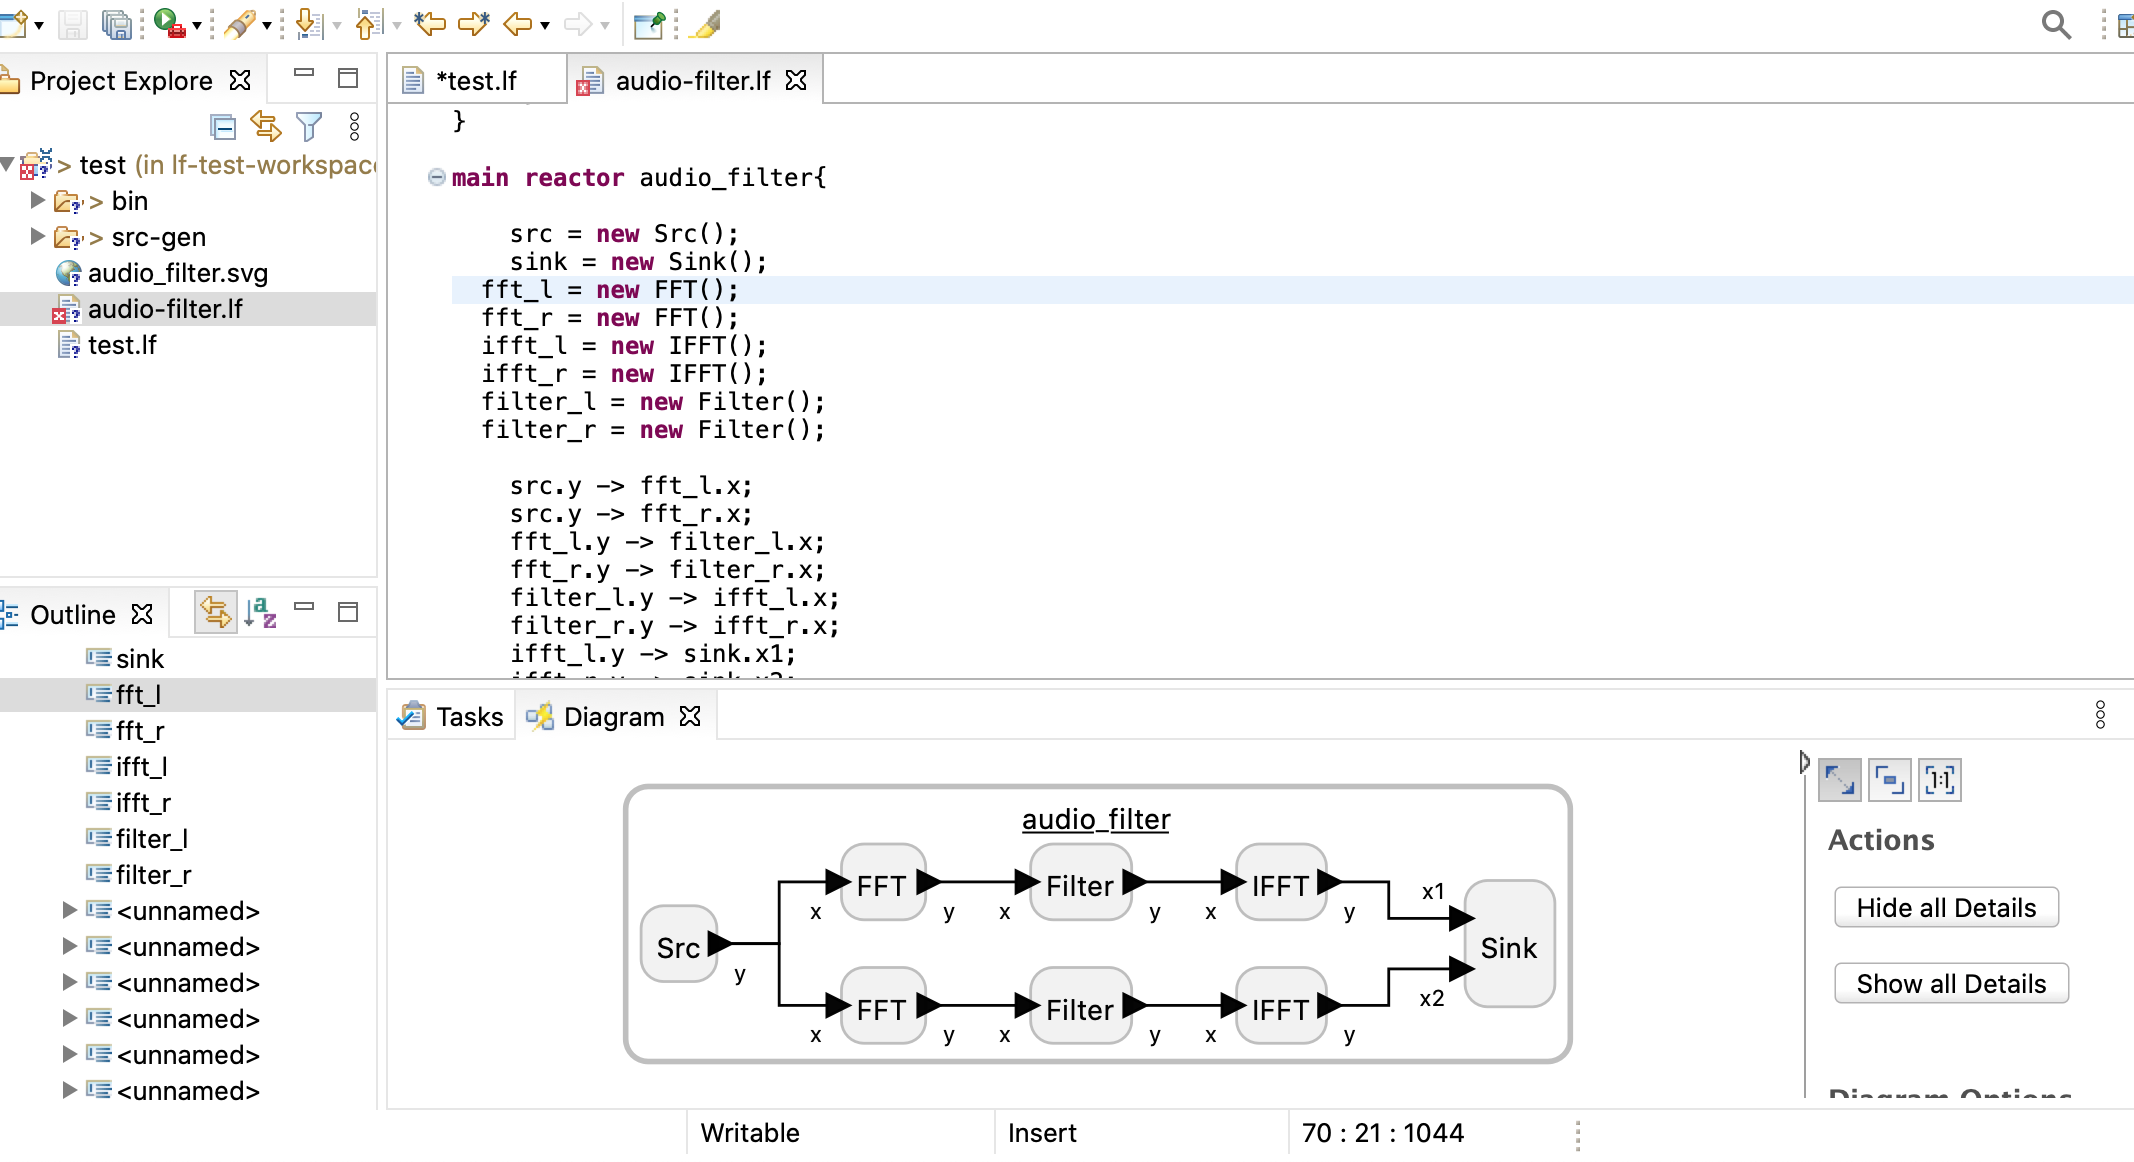
\includegraphics[width=0.9\textwidth]{figures/audio_filter_lf_screenshot.png}
	\caption{The audio filter example in Lingua Franca}
	\label{fig:audio_filter_lf}
	%	\vspace{-1mm}
\end{figure}


\subsection{Implicit Dataflow}

The languages surveyed so far are explicit about their abstractions: Actors, Reactors or Processes are declared explicitly.
Similarly, channels describing the dataflow are made explicit either through channel declarations or through the connection of explicit ports.
A programmer writing in e.g. \ac{CPN} or Lingua Franca has to have a model of the network describing the application in their head (or in their \acs{IDE}).
Implicit abstractions, on the other hand, work by generating implicit models from linguistic constructs that don't exhibit their structure directly.

Implicit abstractions as we just defined them are ubiquitous in programming languages.
Again, objects in \ac{OOP} are an implicit abstraction for data encapsulation that is fundamentally similar to actors.
A thorough classification  of these implicit models is outside the scope of this thesis.
Instead, we will look closely at the Ohua programming paradigm~\cite{ertel_phdthesis}, which derives a dataflow execution from functional semantics.

The Ohua programming model by S. Ertel and others is a powerful model of implicit parallelism which can be used to express parallelism at a language level without explict costructions like threads and locks. 
\index{Ohua}
As stated above, the parallelism comes from lowering an Ohua program into a dataflow-based execution.
This model is not part of the original contribution of this thesis.
However, it is central to several distinct original contributions of the thesis, and we will introduce it as background material.

Ohua itself is a general paradigm that works on multiple language, and the framework has evolved over the years of its development.
The version of Ohua we will discuss here first is based on Clojure and Java, but the Ohua compiler and its principles work with many languages,
and rutimes also exist at different levels of development e.g. for Rust, Javascript or Go.
Ohua is best understood by diving directly into examples. Consider the code in Listing~\ref{listing:ohua_audio_filter}.

\begin{listing}
\begin{minted}[linenos]{Clojure}
 ;; TODO: add the audio filter solution code.
 (ns wav-transform.core
  (:gen-class)
  (:import WavTransform))

(defn -main
  "I don't do a whole lot ... yet."
  [& args]
  (WavTransform/fromFile "oxp.wav" "oxp-transformed.wav")) 
\end{minted}
\caption{The Audio Filter Example written in Ohua}
\label{listing:ohua_audio_filter}
\end{listing}

Listing~\ref{listig:ohua_audio_filter} is based on Clojure, a dialect of Lisp.
It implements the same example from Chapter~\ref{chap:mapping} (cf. Listing~\ref{listing:audio_filter} or Figure~\ref{fig:audio_filter_graph}), a two-channel audio filter.
Internally, the compiler transforms this code into a dataflow graph for execution.
As a \ac{MoC}, this can be embeded in the Dennis dataflow models discussed in Chapter~\ref{chap:mocs}.
We will discuss the semantics of these dataflow graphs in Section~\ref{sec:ohua_dataflow}.
\todo{discuss example}.

The example in Figure~\ref{fig:ohua_example} can be transformed into a dataflow graph for execution. We will discuss this further in Section~\ref{sec:ohua_dataflow}.
The main advantage of this transformation is that a dataflow graph exposes concurrency, which can be exploited e.g. in a parallel execution or for optimizing \ac{I/O}(cf. Section~\ref{sec:yauhau}).
This duality between code and dataflow graphs is a core concept behind Ohua.
The other central pilar of the Ohua design concept are stateful functions, an abstraction that encapsulates functions with state and side-effects in the context of their dataflow execution.
\index{Ohua ! stateful functions}

\subsection{Stateful Functions}
The functional programming community has made the distinction between \emph{pure} and \emph{impure} functions widespread.
A pure function is a function in the mathematical sense of the word: it receives a certain input and, deterministically, produces an output.
This could be as simple as negating a boolean value, or as complicated as inference with a gargantuan deep neural network.
The main point is that the entirety of the usage of a function is that it returns a value in a deterministic fashion from its inputs.

In most imperative languages, like C or Java, functions usually also have side-effects. Writing the output to the terminal, storing data in a global data structure or even reading data from a sensor in a \ac{CPS}, these are all examples of side effects.
A language that only allows pure functions is basically useless, since even printing the result of a computation is impure.
Time is also fundamentally part of a computation, as we have discussed in Chapter~\ref{chap:mocs}, as can be an interaction with the outside world in the form of sensing and actuation in \acp{CPS}.

Stateful functions are a special abstraction, where the concept of pure functions is extended to consider the state of the computation. 
While this excludes aspects like the time of the computation and side-effects like actuation, it is general enough to cover large classes of functions used in most software.
A stateful function is a function $f : a \rightarrow b$ and an abstract state $S$, where the execution of the function can be seen as dependent of the state, which it also modifyies.
In other words, we consider $f$ as a function:
\begin{align}
  f : a \times S \rightarrow b \times S \label{eqn:state_thread}
\end{align}

Pure functions can be seen as a special case of stateful functions, with a trivial state $S = \{*\}$.

\begin{listing}
\begin{minted}[]{Java}
public class ParseVariable{
  @defsfn
  public ParseVariable (ExpressionObject expr, SymbolTable table){
    symbols = expr.parse();
    table.write(symbols);
    return(object);
  }
}
\end{minted}
\caption{An example of a stateful function.}
\label{listing:stateful_function}
\end{listing}


Listing~\ref{listing:stateful_function} shows an example of a stateful function, written in Java, which is identified as such by the \texttt{@defsfn} annotation.
TODO: Discuss (or improve) the example. Admittedly, I'm a bit confused by this, does the state have to be explicit as an input?
By anotating a function as stateful and being able to reason about its state, we can ensure its semantics are preserved when transforming to a dataflow execution.
Traditionally, stateful functions in Ohua are explicitly annotated as such~\cite{ertel_pmam18}.

\subsection{Dataflow Execution}
\label{sec:ohua_dataflow}


Figure~\ref{fig:ohua_example_df} depicts this example as a dataflow graph.
\todo{discuss dataflow graph}.


Ohua

The Ohua framework is based on these two design principles, yet the implementation has constantly evolved since its original inception~\cite{ertel2014framework}.
The work we will present in this chapter played a role in Ohua's evolution.
For this reason, we will discuss the concrete language and transformations in the context they were developed, instead of the latest instantiation of Ohua.

The concepts of Ohua itself and the implementation of the compiler are beyond the scope of this thesis. 
The rest of this chapter will focus mostly on formalizing the semantics and defining semantics-preserving transformations. 
Note that is the joint contribution of a collaborative work with multiple co-authors in~\cite{goens_multiprog18,ertel_cc18,ertel_haskell19,ertel_haskellsup19}.